\documentclass[japanese,draft]{jssst_ppl} %% 日本語 (default)
% \documentclass[english]{jssst_ppl} %% English
% \documentclass[japanese,draft]{jssst_ppl} %% You can use the draft option

\usepackage{ipsj}
\usepackage{color}
\usepackage{amssymb}
\usepackage{amsmath}
\usepackage{amsthm}
\usepackage{multirow,bigdelim}
\newcommand{\la}{\leftarrow}
\newcommand{\Lra}{\Longrightarrow}
\newcommand{\Lla}{\Longleftarrow}
\newcommand{\Llra}{\Longleftrightarrow}
\newcommand{\lra}{\longrightarrow}
\newcommand{\dd}{\mathop{..}}
\newcommand{\range}[2]{\{#1\dd#2\}}
\newcommand{\imp}{\Rightarrow}
\newcommand{\equ}{\Leftrightarrow}
\renewcommand{\labelenumi}{(\arabic{enumi})}
\newcommand{\alldiff}{\textrm{alldifferent}}
\newcommand{\Alldiff}{\alldiff(x_1,x_2,\ldots,x_n)}
\newcommand{\SAT}{{\tt SAT}}
\newcommand{\UNSAT}{{\tt UNSAT}}
\newcommand{\Dom}{{\it Dom}}
% \newcommand{\p}[2]{p(#1,#2)}
\newcommand{\dE}[2]{p(#1=#2)}
\newcommand{\lE}[2]{p(#1^{(#2)})}
\newcommand{\oE}[2]{p(#1\le#2)}


\title{解集合プログラミングを用いた配電網問題の解法}
\author{山田 健太郎$^1$,湊 真一$^2$,田村 直之$^3$,番原 睦則$^4$}
\inst{%
$^1$ 名古屋大学大学院 情報学研究科\\
\texttt{yken66@nagoya-u.jp}
\medskip\par%所属の区切り
$^2$ 京都大学大学院 情報学研究科\\
\texttt{minato@i.kyoto-u.ac.jp}
\medskip\par%所属の区切り
$^3$ 神戸大学 情報基盤センター\\
\texttt{tamura@kobe-u.ac.jp}
\medskip\par%所属の区切り
$^4$ 名古屋大学大学院 情報学研究科\\
\texttt{banbara@nagoya-u.jp}
}
\begin{document}
\maketitle
\begin{abstract}
%%%%%%%%%%%%%%%%%%%%%%%%%%%%%%%%%%%%%%%%%%%%%%%%%%%%%%%%%%% 
\chapter*{概要}
\pagenumbering{roman}
%%%%%%%%%%%%%%%%%%%%%%%%%%%%%%%%%%%%%%%%%%%%%%%%%%%%%%%%%% 

% 表紙を情報工学コース用のスタイルにするために,作成した{\tt jbachelor.sty}が
% 必要である.
% TexStudioなどの便利なTex統合環境を利用するために,lualtexを使うとよい.
% platex と lualatex を切り替えるためには,このファイルの先頭を編集してlualatex用
% のltjbook.clsを使うようにする.
% \begin{verbatim}
% %%% for platex
% \documentclass[a4paper,12pt]{jbook}
% %%% for lualatex
% %\documentclass[a4paper,12pt]{ltjbook}
% \end{verbatim}

% 命題論理の充足可能性判定問題(Boolean SATisfiability; SAT)は,与えられ
% た命題論理式の充足可能性を判定する問題である.
% 近年,SAT の解を求める SAT ソルバーの性能が大きく向上し,
% SAT を拡張・発展させた問題を中心に,SAT 技術が大きな広がりを見せている.
%
% なかでも,
背景理論付き SAT (Satisfiability Modulo Theories; SMT) は,
背景理論が扱えるよ
うに,SAT を拡張・発展させた技術である.
SMT は,背景理論をより表現能力の高い述語論理で記述できるため,
問題を簡潔に記述することができる点が特長である.
% 近年,SAT ソルバー
% を拡張した高速 SMT ソルバーが開発され,制約充足問題,プログラム検証な
% どへの応用が活発に研究されている.

制約プログラミングの言語である制約充足問題は,与えられた制約を満たす解
を探索する問題である.
制約充足問題では,グローバル制約を用いて,複数の変数に対する複雑な
制約を簡潔に表現できる点が特長の一つである.
代表的なグローバル制約$distinct(x_{1},x_{2},\ldots x_{n})$は,
$x_{i}$が互いに異なる値をとることを表す.
この$distinct$制約は,記述性の向上を目的として SMT ソルバー
にも取り入れられている.
しかしながら,制約充足問題に対する SMT ソルバーの求解性能は,
SAT 型制約ソルバーと比べて劣っているとの報告もあり,
$distinct$制約を含めその効率的な実装は重要な研究課題となっている.

本論文では,クイーングラフ彩
色問題を題材とし,その SMT 符号化と$distinct$制約の高速化について述べる.
クイーングラフ彩色問題の SMT 符号化として,
色変数モデル,位置変数モデル,0-1変数モデル,ハイブリッドモデルを実装した.
また,$distinct$制約の高速化として,
色変数モデルと位置変数モデルでは,
SAT型制約ソルバーで有効性が示されている鳩の巣原理等に基づくヒント制約を追加した.
0-1変数モデルとハイブリッドモデルでは,
$distinct$制約のPB符号化[大野,2019]を応用し,探索空間の枝刈りを実装した.

クイーングラフ彩色問題($5\leq N \leq 13$)を用いた実行実験の結果,
色変数モデル+ヒント制約と位置変数モデル+ヒント制約が,$N=11$まで解を求め,最も良い性能を示した.
これにより,$distinct$制約の高速化について,
SATでのヒント制約が SMT においても有効であることが確認できた.
その一方で,チャネリング制約を用いたハイブリッドモデルは,
SMTソルバーの場合,求解性能が低下することが確認された.

%%% Local Variables:
%%% mode: japanese-latex
%%% TeX-master: "paper"
%%% End:

\end{abstract}

%%%%%%%%%%%%%%%%%%%%%%%%%%%%%%%%%%%%%%%%%%%%%%%%%%%%%%%%%% 
\chapter{緒論}

\pagenumbering{arabic}

\textbf{時間割問題} (Timetabling Problem) は,
求解困難な組合せ最適化問題の一種である.
この問題には,ハード制約とソフト制約が存在し,ソフト制約に違反するとペ
ナルティが与えられる.必ず満たすべきハード制約を満たしながら,ペナルティ
の総和を最小にするような解を求めることが目的である.
現状では,質の高い時間割を編成するために多くの人間の労力が費やされている.
このような背景から,時間割に関する国際会議
(Practice and Theory of Automated Timetabling; PATAT)
や国際時間割競技会 (International Timetabling Competition; ITC)
が開催され,時間割ソルバーの性能向上に貢献している.

\textbf{解集合プログラミング} (Answer Set Programming; ASP) 
\cite{%
  Baral03:cambridge,%
  Gelfond88:iclp,%
  Inoue08:jssst,%
  Niemela99:amai}
  は,
論理プログラミングから派生した宣言的プログラミングパラダイムの一つである.
ASP 言語は一階論理に基づく知識表現言語の一種であり,論理プログラムは
ASP のルールの有限集合である.ASP システムは論理プログラムから安定モデ
ル意味論に基づく解集合を計算するシステムである.
近年,SAT 技術を応用した高速 ASP システムが実現され,ロボット工学,シ
ステム生物学,システム検証,プランニングなど様々な分野への実用的応用が
急速に拡大している.

近年,\textbf{カリキュラムベース・コース時間割}
(Curriculum-based Course Timetabling; CB-CTT)
問題に対する ASP を用いた解法が提案され,成功を収めている
\cite{%
 banbara17:ramp}.
CB-CTT 問題は,大学等の1週間の講義スケジュールを求める問題であり,
最も研究が盛んな教育時間割問題の一つである.
ASP は系統的探索であることを活かして,未解決問題の最適値を決定するなど
優れた性能を示している.
しかし,その一方で,ソフト制約が多く含まれるような問題集において,
局所的探索を用いた解法より性能が劣っている場合が見られる.

この問題を解決するために,系統的探索と局所的探索を組み合わせた
\textbf{Large Neighborhood Prioritized Search} (LNPS)
\cite{%
 hayama19:kobe}
が提案されている.
LNPS は,暫定解に含まれる変数の値割り当ての一部をランダムに選んで取り
消し,他の値割り当てをなるべく維持したままで解を再構築する反復法の一種
である.
ASP を用いた LNPS の利点は,解の再構築を系統的探索で行え,値割り当てを
なるべく維持したままでの再構築が自然に実現できることである.
LNPS の性能は,
暫定解の一部をランダムに選んで取り消す destroy 演算子に依存するが,
十分な研究がなされてない.

本論文では,LNPS を用いたカリキュラムベース・コース時間割 (CB-CTT)
問題の解法について述べる.
CB-CTT に対する既存研究
\cite{%
 kiefer16:patat}
 を応用して,
3種類の destroy 演算子 (random, day-period, day-room) を実装した.
random が問題の性質をまったく利用しないのに対し,
day-period と day-room は CB-CTT のソフト制約を考慮して
暫定解の一部をランダムに選んで取り消す点が特長である.
%
提案手法の有効性を評価するために,国際時間割競技会 ITC-2007 のベンチマー
ク問題(21問)を用いて実行実験を行った.その結果,
多くの問題に対して,day-period と day-room が既存 ASP 解法より良い解を
生成し,提案手法の有効性が確認できた.

以降の構成は以下の通りである.
第二章で時間割問題,特に本論文が対象とするカリキュラムベース・コース時
間割問題について述べる.
第三章で解集合プログラミングについて述べ,その中で,LNPS の実装におい
て重要な変数選択ヒューリスティクスの変更機能について述べる.
第四章で LNPS 及び 実装した destroy 演算について述べる.
第五章でカリキュラムベース・コース時間割問題に実装解法を適用した実験の
結果を述べ,既存 ASP との比較や,destroy 演算同士での比較を交え考察を
行う.
最後に第六章で結論を述べる.

%%%%%%%%%%%%%%%%%%%%%%%%%%%%%%%%%%%%%%%%%%%%%%%%%%%%%%%%%% 


%%% Local Variables:
%%% mode: latex
%%% TeX-master: "paper"
%%% End:

\section{配電網問題と配電網遷移問題}\label{chap:problem}

%\subsection{配電網問題}

配電網問題は,
与えられた配電網$D=(S,SW)$から,以下の制約(\ref{topology}), (\ref{electrical})を満たす
配電網の構成(スイッチの開閉状態)が存在するかどうかを判定する問題である.
$S$は配電区間を表すセクションの集合,
$SW$は配電区間を結ぶスイッチの集合である.
本論文では,配電網の構成を閉じたスイッチの集合$X\subset SW$で表す.
すなわち,$X$がこの問題の実行可能解である.
$I_{i}$は各セクション$s_{i}\in S$の電流,
$J^{max}$はセクションにおける許容電流を表し,
ともに入力として与えられる.
% 
\begin{eqnarray}
& X ~\textrm{によって定まる配電網構成に停電と短絡が発生しない}   \label{topology}\\
% & J_i = \displaystyle\sum_{j\in S_i^{down}} I_j \qquad (\forall s_{i}\in S)\nonumber\\
% & J_i \leq J_{i}^{max} \qquad (\forall s_{i}\in S)\label{electrical}
& J_i = \displaystyle\sum_{j\in S_i^{down}} I_j, \qquad J_i \leq J^{max}
  \qquad (\forall s_{i}\in S)\label{electrical}
\end{eqnarray}
%

制約~(\ref{topology})は\textbf{トポロジ制約}と呼ばれる.
トポロジ制約を満たす配電網構成は,配電網$D$に対応するグラフから,
\textbf{根付き全域森}と呼ばれる部分グラフを求める問題に帰着できる~\cite{Minato:dnet:netuki}.
直観的には,セクションがノード,スイッチが辺,変電所が根ノードに対応する.
根付き全域森の定義は以下の通りである.

\theoremstyle{definition}
\newtheorem*{definition*}{定義}
\begin{definition*}
  グラフ$G=(V,E)$と,根と呼ばれる$V$上のノードの集合が与えられたとする.
  このとき,$G$上の根付き全域森とは,以下の制約を満たす$G$の部分グラフ
  $G'=(V,E'), E' \subseteq E$ である.
  \begin{itemize}
  \item $G'$はサイクルを持たない.(非閉路制約)
  \item $G'$の各連結成分は,ちょうど1つの根を含む.(根付き連結制約)
  \end{itemize}
\end{definition*}

制約~(\ref{electrical})は\textbf{電流制約}と呼ばれる.
$S_{i}^{down}$は,各セクション$s_{i}$に対して,自身を含む
下流のセクションの集合を表す.
$J_{i}$はセクション$s_{i}$およびその下流の電流の総和を表し,
許容電流$J^{max}$以下でなければならない.
%
上で述べた配電網問題の定義は,論文~\cite{Minato:dnet:ZDD}に基づいている.
論文~\cite{Minato:dnet:ZDD}では
配電損失を最小にする最適化問題として定義されている.
本論文では,後で述べる配電網遷移問題への拡張を主眼とするため,
配電網問題を判定問題として定義している.

%%%%%%%%%%%%%%%%%%%%%%%%%%%%%%%
\begin{figure}[tb]
 \centering
 \scalebox{0.6}{%%%%%%%%%%%%%%%%%%%%%%%%%%%%%%%%%%%%%%%%%%%%%%%%%%
% 配電網 例 (第1章で使う)
%%%%%%%%%%%%%%%%%%%%%%%%%%%%%%%%%%%%%%%%%%%%%%%%%%

\begin{tikzpicture}

 % setting
 \tikzset{customer/.style={rectangle,thick,draw=black,minimum size=0.5cm}}
 \tikzset{on_switch/.style={rectangle,fill=black}}
 \tikzset{off_switch/.style={rectangle,draw=black,fill=white}}
 
 \tikzset{node distance =1cm};

 % substation (x, y, label)
 \newcommand{\substation}[3]{
 \draw [very thick] (#1,#2) circle [radius=0.225cm] node[draw=white,minimum size=1cm](#3){};
 \draw [very thick] (#1+0.225,#2)--(#1+0.35,#2)--(#1+0.35,#2+0.3);
 \draw [very thick] (#1-0.225,#2)--(#1-0.35,#2)--(#1-0.35,#2-0.3);
 \draw [very thick] (#1,#2+0.225)--(#1,#2+0.35);
 \draw [very thick] (#1,#2-0.225)--(#1,#2-0.35);
 \draw [very thick] [domain=-0.284:-0.159] plot(\x+#1,\x+#2);
 \draw [very thick] [domain=0.159:0.284] plot(\x+#1,\x+#2);
 \draw [very thick] [domain=-0.284:-0.159] plot(\x+#1,-\x+#2);
 \draw [very thick] [domain=0.159:0.284] plot(\x+#1,-\x+#2);
 }

 %switch node (position, label, cap)
 %% right switch
 \newcommand{\swnodeR}[4]{
 \coordinate[#1] (#2);
 \node[#1,customer] (#2){#4};
 \node[circle, draw=black, text width=0.2cm, 
 right=0cm of #2, scale=0.3, thick] {};
 \node[right=0cm of #2,scale=0.3, minimum size=0.8cm] (#3){};
 }
 %% left switch
 \newcommand{\swnodeL}[4]{
 %\coordinate[#1] (#2);
 \node[#1,customer] (#2){#4};
 \node[circle, draw=black, fill=white, text width=0.2cm, 
 left=0cm of #2, scale=0.3, thick] (#3){};
 }
 % above switch
 \newcommand{\swnodeA}[4]{
 \coordinate[#1] (#2);
 \node[#1,customer] (#2){#4};
 \node[circle, draw=black, text width=0.2cm, 
 above=0cm of #2, scale=0.3, thick] (#3){};
 }
 % below switch
 \newcommand{\swnodeB}[4]{
 \coordinate[#1] (#2);
 \node[#1,customer] (#2){#4};
 \node[circle, draw=black, text width=0.2cm, 
 below=0cm of #2, scale=0.3, thick] {};
 \node[below=0cm of #2,scale=0.3,minimum size=0.8cm] (#3){};
 }
 
 \substation{0}{0}{sub};
 
 % root1
 \node[customer,fill=black!40,below =4.5cm of sub] (root1) { };
 \swnodeL{left =of root1}{node1}{sw1}{ };
 
 \swnodeR{left=of node1}{node2}{sw2}{ };
 \node[customer,left=of node2] (junc1){ };
 \swnodeL{left =of junc1}{node3}{sw3}{ };
 \swnodeA{above= of junc1}{node4}{sw4}{ }

 \swnodeR{left=of node3}{node5}{sw5}{ };
 \swnodeA{above =of node5}{node6}{sw6}{ };

 \swnodeB{above =of node6}{node7}{sw7}{ };
 \swnodeA{above =of node7}{node29}{sw29}{ };

 \swnodeB{above =of node29}{node30}{sw30}{ };
 
 \swnodeB{above =of node4}{node8}{sw8}{ };
 \swnodeA{above =of node8}{node31}{sw31}{ };
 
 \swnodeB{above =of node31}{node32}{sw32}{ };

 \swnodeR{right =of root1}{node17}{sw17}{ };

 \swnodeL{right =of node17}{node18}{sw18}{ };

 % root2
 \node[customer,fill=black!10,above=4.5cm of sub] (root2) { };
 \swnodeL{left =of root2}{node9}{sw9}{ };

 \swnodeR{left=of node9}{node10}{sw10}{ };
 \node[customer,left=of node10] (junc2){ };
 \swnodeL{left =of junc2}{node11}{sw11}{ };
 \swnodeB{below =of junc2}{node12}{sw12}{ };
 
 \swnodeR{left =of node11}{node13}{sw13}{ };
 \swnodeB{below =of node13}{node14}{sw14}{ };
 
 \swnodeA{below =of node14}{node15}{sw15}{ };

 \swnodeA{below =of node12}{node16}{sw16}{ };

 \swnodeR{right =of root2}{node22}{sw22}{ };

 \swnodeL{right =of node22}{node23}{sw23}{ };
 
 % root3
 \node[customer,pattern=north east lines,right=5.2cm of sub] (root3) { };
 \swnodeB{below =1.4of root3}{node24}{sw24}{ };
 \swnodeA{above =1.4of root3}{node25}{sw25}{ };

 \swnodeA{below =of node24}{node19}{sw19}{ };
 \swnodeL{below =1.3of node19}{node20}{sw20}{ };
 
 \swnodeR{left =of node20}{node21}{sw21}{ };

 \swnodeB{above =of node25}{node26}{sw26}{ };
 \swnodeL{above =1.3of node26}{node27}{sw27}{ };

 \swnodeR{left =of node27}{node28}{sw28}{ };
 
 % sections
 \foreach \v / \u / \t in {root1/sub/$s_a$,root1/node1/$s_1$,node2/junc1/$s_2$, %
 junc1/node3/$s_3$,junc1/node4/$s_4$,node5/node6/$s_5$,node7/node29/$s_6$,node30/node15/$s_7$, %
 sub/root2/$s_b$,root2/node9/$s_8$,node10/junc2/$s_9$,junc2/node11/$s_{10}$,node12/junc2/$s_{11}$, %
 node14/node13/$s_{12}$,node8/node31/$s_{13}$,node32/node16/$s_{14}$,node17/root1/$s_{15}$, %
 node22/root2/$s_{16}$,root3/sub/$s_c$,node24/root3/$s_{17}$,root3/node25/$s_{18}$, %
 node20/node19/$s_{19}$,node26/node27/$s_{20}$,node21/node18/$s_{21}$,node28/node23/$s_{22}$} %
 \draw[thick] (\v) --  node[auto=right]{\t} (\u);

 % switches
 %% horizontal
 \foreach \v / \u / \t in {sw1/sw2/$sw_{1}$,sw3/sw5/$sw_{2}$,sw9/sw10/$sw_{11}$,sw11/sw13/$sw_{12}$,sw18/sw17/$sw_{13}$,
 sw23/sw22/$sw_{15}$,sw20/sw21/$sw_{14}$,sw27/sw28/$sw_{16}$}
 \draw[very thick] (\v) -- node[below=0.2of \v]{\t} (\u.45);
 %% vertical
 \foreach \v / \u / \t in {sw4/sw8/$sw_{4}$,sw6/sw7/$sw_{3}$,sw29/sw30/$sw_{5}$,sw31/sw32/$sw_{6}$,sw15/sw14/$sw_{7}$,%
 sw16/sw12/$sw_{8}$,sw19/sw24/$sw_{9}$,sw25/sw26/$sw_{10}$}
 \draw[very thick] (\v) -- node[auto=below]{\t~~~~~~~~~~} (\u.-30);

\end{tikzpicture}

%%%%%%%%%%%%%%%%%%%%%%%%%%%%%%%%%%%%%%%%%%%%%%%%%%%%%%%%%%
%%% Local Variables:
%%% mode: japanese-latex
%%% TeX-master: paper.tex
%%% End:
}
  \caption{配電網問題の例}
  \label{fig:test-input}
\end{figure}
%%%%%%%%%%%%%%%%%%%%%%%%%%%%%%%
% %%%%%%%%%%%%%%%%%%%%%%%%%%%%%%%
% \begin{table}[tbp]
%  \centering
%  \caption{負荷電流の一覧~(A)}
%  \label{table:current}
%  \begin{tabular}{ccc|ccc|ccc|ccc|ccc}
 \noalign{\hrule height 1pt}
 $I_{a}$ &=& 16 & $I_{b}$ & = & 41 & $I_{c}$ & = & 16 & $I_{1}$ & = & 40 & $I_{2}$ & = & 5 \\
 $I_{3}$ & = & 34 & $I_{4}$ & = & 0 & $I_{5}$ & = & 11 & $I_{6}$ & = & 34 & $I_{7}$ & = & 24 \\
 $I_{8}$ & = & 31 & $I_{9}$ & = & 45 & $I_{10}$ & = & 24 & $I_{11}$ & = & 0 & $I_{12}$ & = & 45 \\
 $I_{13}$ & = & 21 & $I_{14}$ & = & 20 & $I_{15}$ & = & 0 & $I_{16}$ & = & 0 & $I_{17}$ & = & 0 \\
 $I_{18}$ & = & 0 & $I_{19}$ & = & 35 & $I_{20}$ & = & 20 & $I_{21}$ & = & 35 & $I_{22}$ & = & 20 \\
 \noalign{\hrule height 1pt}
\end{tabular}
% \end{table}
% %%%%%%%%%%%%%%%%%%%%%%%%%%%%%%%
%%%%%%%%%%%%%%%%%%%%%%%%%%%%%%%%%%%%% 
\begin{figure}[tb]
 \centering
 \scalebox{0.6}{\input{tikz/tikz-test-output}}
 \caption{配電網問題(図\ref{fig:test-input})の解の一例}
 \label{fig:test-output}
\end{figure}
%%%%%%%%%%%%%%%%%%%%%%%%%%%%%%%%%%%%% 

%%%%%%%%%%%%%%%%%%%%%%%%%%%%%%%%%%%%% 
\begin{figure}[tbp]
  \centering
  \scalebox{0.8}{%%%%%%%%%%%%%%%%%%%%%%%%%%%%%%%%%%%%%%%%%%%%%%%%%%
% 根付き全域森 (第2章で使う)
%%%%%%%%%%%%%%%%%%%%%%%%%%%%%%%%%%%%%%%%%%%%%%%%%%

\begin{tikzpicture}[x=1.5cm,y=1.5cm,scale=0.7]

 % 設定
 \tikzset{root/.style={circle,draw=black,fill=gray!30,minimum size=1cm}}
 \tikzset{node/.style={circle,draw=black,minimum size=1cm}}
 
 % 補助線
 % \draw [help lines,blue,step=2cm] (-3,0) grid (3,-3);


 \node[node,fill=purple!60,label=above:$r_1$] (r1){$1$};

 \node[node,fill=purple!60,left=of r1] (n1){$5$};
 \node[node,fill=purple!60,left=of n1] (n2){$4$};
 \node[node,fill=cyan!80,above=of n2] (n3){$6$};
 \node[node,fill=purple!60,above=of n1] (n4){$8$};
 \node[node,fill=cyan!80,above=of n3] (n5){$8$};
 \node[node,fill=cyan!80,above=of n4] (n6){$9$};
 \node[node,fill=cyan!80,above=of n5] (n7){$10$};
 \node[node,fill=cyan!80,above=of n6] (n8){$11$};

 \node[node,fill=cyan!80,right=of n8,label=above:$r_2$] (r2){$2$};
 \node[node,fill=cyan!80,right=of r2] (n9){$14$};
 \node[node,fill=yellow!80,right=of n9] (n10){$15$};
 \node[node,fill=purple!60,right=of r1] (n11){$12$};
 \node[node,fill=yellow!80,right=of n11] (n12){$13$};
 
 \node[node,fill=yellow!80,label=right:$r_3$](r3) at ($(n10)!0.5!(n12)$) {$3$};
 
 \foreach \v / \u in {r1/n1,n1/n2,n1/n4,n3/n5,n5/n7,n6/n8,n7/n8,n8/r2,
 r2/n9,r1/n11,r3/n10,r3/n12}
 \draw[thick] (\v) -- (\u);

\end{tikzpicture}

%%%%%%%%%%%%%%%%%%%%%%%%%%%%%%%%%%%%%%%%%%%%%%%%%%%%%%%%%%
%%% Local Variables:
%%% mode: japanese-latex
%%% TeX-master: paper.tex
%%% End:
}
  \caption{配電網問題の解(図\ref{fig:test-output})に対応する根付き全域森}
  \label{fig:test-netsuki-output}
\end{figure}  
%%%%%%%%%%%%%%%%%%%%%%%%%%%%%%%%%%%%%

DNET
% \footnote{\url{https://github.com/takemaru/dnet}}
に公開されている配電網問題の例を図~\ref{fig:test-input}に示す.
この例は,
25箇所のセクション$S=\{s_{a},s_{b},s_{c},s_{1},\ldots, s_{22}\}$,
16個のスイッチ$SW=\{sw_{1},\ldots, sw_{16}\}$,
3箇所の変電所$\{s_{a}, s_{b}, s_{c}\}$
から構成されている.
ここでは,変電所に直接つながるセクションをそれぞれ変電所とする.
%
図\ref{fig:test-output}に,この配電網問題の解の一例を示す.
閉じたスイッチは,
\[X=\{sw_{1},sw_{2},sw_{4},sw_{5},sw_{7},sw_{8},sw_{9},%
sw_{10},sw_{11},sw_{12},sw_{13},sw_{15}\}\]
となる.
変電所$s_{a}$から電力の供給を受けるセクションの端点を赤色で,
変電所$s_{b}$からを青色で,
変電所$s_{c}$からを黄色で表している.
トポロジ制約を満たし,停電と短絡が発生しないことがわかる.
図\ref{fig:test-output}の配電網問題の解に対応する根付き全域森を
図\ref{fig:test-netsuki-output}に示す.
例えば,セクション\{$s_a,s_1,s_{15}$\}は,ノード1に対応し,
変電所$s_a,s_b,s_c$に対応する各ノードは,根$r_1,r_2,r_3$にそれぞれ対応する.
また,電流制約について,例えば,セクション$s_2$の下流にあるセクションの
集合は,$S_2^{down}=\{s_{2},s_{3},s_{4},s_{5},s_{13}\}$となる.したがって,
$J_{2}=I_{2}+I_{3}+I_{4}+I_{5}+I_{13}$のように計算される.


% 次に例として,図\ref{fig:test-input}で示した配電網問題の解を図\ref{fig:test-output}に示す.
% この解は電流制約を$V_{max}=300$として求められた解である.閉じたスイッチは,$\{sw_{1},sw_{2},
% sw_{4},sw_{5},sw_{7},sw_{8},sw_{9},sw_{10},sw_{11},sw_{12},sw_{13},sw_{15}\}$である.
% このスイッチの集合から決まる配電経路は,図\ref{fig:test-output}の通り,トポロジ制約を満たしている.
% また,各変電所に$\{s_a,s_b,s_c\}$について,それぞれ,
% $s_a^{down}=\{s_a,s_1,s_2,s_3,s_4,s_5,s_{13},s_{15},s_{21}\}$,
% $s_b^{down}\{s_b,s_6,s_7,s_8,s_9,s_{10},s_{11},s_{12},s_{14},s_{16},s_{22}\}$,
% $s_c^{down}=\{s_c,s_{17},s_{18},s_{19},s_{20}\}$である.
% したがって,表\ref{table:current}より,各供給経路に対する電流値の合計は,$J_a=162$,$J_b=284$,$J_c=71$となり,
% 電流制約も満たしている.

% ここで,トポロジ制約を満たす配電網構成は,\textbf{根付き全域森}という部分グラフに対応する
% ことが知られている~\cite{Minato:dnet:netuki}.
% 根付き全域森は以下のように定義される.
% \theoremstyle{definition}
% \newtheorem*{definition*}{定義}
% \begin{definition*}
%   グラフ$G=(V,E)$と,根と呼ばれる$V$上のノードの集合が与えられたとする.
%   このとき,$G$上の根付き全域森とは,以下の制約を満たす$G$の部分グラフ
%   $G'=(V,E'), E' \subseteq E$ である.
%   \begin{enumerate}
%   \item $G'$はサイクルを持たない.(非閉路制約)
%   \item $G'$の各連結成分は,ちょうど1つの根を含む.(根付き連結制約)
%   \end{enumerate}
% 本稿では,与えられたグラフ$G$から,根付き全域森
% $G'$を求める部分グラフ探索問題を\textbf{根付き全域森問題}と呼ぶ.
% \end{definition*}

% 根付き全域森問題の入力例となるグラフを図\ref{fig:test-netsuki-input}に示す.
% 図\ref{fig:test-netsuki-input}は,図\ref{fig:test-input}で示した配電網に対応しており,
% 配電区間$\{s_i ~|~ 1 \leq i \leq 22\}$は,スイッチで区切られる1つのまとまりごとに
% \textbf{ノード}に対応する.例えば,区間$\{s_2,s_3,s_4\}$は,ノード5に対応している.
% スイッチ$\{sw_1,\ldots,sw_{16}\}$は,\textbf{辺}に対応する.
% また,図中の色付きノード$\{r_1,r_2,r_3\}$は変電所を含むことを意味しており,
% \textbf{根}に対応している.

% 根付き全域森の例を図\ref{fig:test-netsuki-output}に示す.根付き全域森は,
% 各連結成分が必ずちょうど1つの根をもつ木構造を形成することで,
% 非閉路制約と根付き連結制約を満たす.図\ref{fig:test-netsuki-output}は,
% 図\ref{fig:test-output}の配電網問題の解に対応している.



%\subsection{配電網遷移問題}

%%%%%%%%%%%%%%%%%%%%%%%%%%%%%%%%%%%%% 
\newcommand{\lw}[1]{\smash{\lower-15.ex\hbox{#1}}}
\begin{figure*}[tb]
  %\renewcommand{\arraystretch}{0.9}
  \tabcolsep = 3mm
  \centering
  \begin{tabular}{ccc}
    $t=0$ (スタート状態) & & $t=1$\\
    \scalebox{0.45}{\input{tikz/tikz-test-core-0}}
    & \lw{$\Rightarrow$} & 
    \scalebox{0.45}{\input{tikz/tikz-test-core-1}}\\
    & & $\Downarrow$\\
    & & \\
    \scalebox{0.45}{\input{tikz/tikz-test-core-3}}
    & \lw{$\Leftarrow$} &
    \scalebox{0.45}{\begin{tikzpicture}

 % setting
 \tikzset{customer/.style={rectangle,thick,draw=black,minimum size=0.5cm}}
 \tikzset{on_switch/.style={rectangle,fill=black}}
 \tikzset{off_switch/.style={rectangle,draw=black,fill=white}}
 
 \tikzset{node distance =1cm};

 % substation (x, y, label)
 \newcommand{\substation}[3]{
 \draw [very thick] (#1,#2) circle [radius=0.225cm] node[draw=white,minimum size=1cm](#3){};
 \draw [very thick] (#1+0.225,#2)--(#1+0.35,#2)--(#1+0.35,#2+0.3);
 \draw [very thick] (#1-0.225,#2)--(#1-0.35,#2)--(#1-0.35,#2-0.3);
 \draw [very thick] (#1,#2+0.225)--(#1,#2+0.35);
 \draw [very thick] (#1,#2-0.225)--(#1,#2-0.35);
 \draw [very thick] [domain=-0.284:-0.159] plot(\x+#1,\x+#2);
 \draw [very thick] [domain=0.159:0.284] plot(\x+#1,\x+#2);
 \draw [very thick] [domain=-0.284:-0.159] plot(\x+#1,-\x+#2);
 \draw [very thick] [domain=0.159:0.284] plot(\x+#1,-\x+#2);
 }

 %switch node (position, label, cap)
 %% right switch
 \newcommand{\swnodeR}[4]{
 \coordinate[#1] (#2);
 \node[#1,customer] (#2){#4};
 \node[circle, draw=black, text width=0.2cm, 
 right=0cm of #2, scale=0.3, thick] {};
 \node[right=0cm of #2,scale=0.3, minimum size=0.8cm] (#3){};
 }
 %% left switch
 \newcommand{\swnodeL}[4]{
 %\coordinate[#1] (#2);
 \node[#1,customer] (#2){#4};
 \node[circle, draw=black, fill=white, text width=0.2cm, 
 left=0cm of #2, scale=0.3, thick] (#3){};
 }
 % above switch
 \newcommand{\swnodeA}[4]{
 \coordinate[#1] (#2);
 \node[#1,customer] (#2){#4};
 \node[circle, draw=black, text width=0.2cm, 
 above=0cm of #2, scale=0.3, thick] (#3){};
 }
 % below switch
 \newcommand{\swnodeB}[4]{
 \coordinate[#1] (#2);
 \node[#1,customer] (#2){#4};
 \node[circle, draw=black, text width=0.2cm, 
 below=0cm of #2, scale=0.3, thick] {};
 \node[below=0cm of #2,scale=0.3,minimum size=0.8cm] (#3){};
 }
 
 \substation{0}{0}{sub};
 
 % root1
 \node[customer,fill=black!40,below =4.5cm of sub] (root1) { };
 \swnodeL{left =of root1,fill=black!40}{node1}{sw1}{ };
 
 \swnodeR{left=of node1,fill=black!40}{node2}{sw2}{ };
 \node[customer,left=of node2,fill=black!40] (junc1){ };
 \swnodeL{left =of junc1,fill=black!40}{node3}{sw3}{ };
 \swnodeA{above= of junc1,fill=black!40}{node4}{sw4}{ }

 \swnodeR{left=of node3,fill=black!40}{node5}{sw5}{ };
 \swnodeA{above =of node5,fill=black!40}{node6}{sw6}{ };

 \swnodeB{above =of node6,fill=black!40}{node7}{sw7}{ };
 \swnodeA{above =of node7,fill=black!40}{node29}{sw29}{ };

 \swnodeB{above =of node29,fill=black!10}{node30}{sw30}{ };
 
 \swnodeB{above =of node4,fill=black!40}{node8}{sw8}{ };
 \swnodeA{above =of node8,fill=black!40}{node31}{sw31}{ };
 
 \swnodeB{above =of node31,fill=black!10}{node32}{sw32}{ };

 \swnodeR{right =of root1,fill=black!40}{node17}{sw17}{ };

 \swnodeL{right =of node17,fill=black!40}{node18}{sw18}{ };

 % root2
 \node[customer,fill=black!20,above=4.5cm of sub, fill=black!10] (root2) { };
 \swnodeL{left =of root2,fill=black!10}{node9}{sw9}{ };

 \swnodeR{left=of node9,fill=black!10}{node10}{sw10}{ };
 \node[customer,left=of node10,fill=black!10] (junc2){ };
 \swnodeL{left =of junc2,fill=black!10}{node11}{sw11}{ };
 \swnodeB{below =of junc2,fill=black!10}{node12}{sw12}{ };
 
 \swnodeR{left =of node11,fill=black!10}{node13}{sw13}{ };
 \swnodeB{below =of node13,fill=black!10}{node14}{sw14}{ };
 
 \swnodeA{below =of node14,fill=black!10}{node15}{sw15}{ };

 \swnodeA{below =of node12,fill=black!10}{node16}{sw16}{ };

 \swnodeR{right =of root2,fill=black!10}{node22}{sw22}{ };

 \swnodeL{right =of node22,fill=black!10}{node23}{sw23}{ };
 
 % root3
 \node[customer,fill=black!20,right=5.2cm of sub,pattern=north east lines] (root3) { };
 \swnodeB{below =1.4of root3,pattern=north east lines}{node24}{sw24}{ };
 \swnodeA{above =1.4of root3,pattern=north east lines}{node25}{sw25}{ };

 \swnodeA{below =of node24,pattern=north east lines}{node19}{sw19}{ };
 \swnodeL{below =1.3of node19,pattern=north east lines}{node20}{sw20}{ };
 
 \swnodeR{left =of node20,fill=black!40}{node21}{sw21}{ };

 \swnodeB{above =of node25,fill=black!10}{node26}{sw26}{ };
 \swnodeL{above =1.3of node26,fill=black!10}{node27}{sw27}{ };

 \swnodeR{left =of node27,fill=black!10}{node28}{sw28}{ };
 
 % sections
 \foreach \v / \u / \t in {root1/sub/$s_a$,root1/node1/$s_1$,node2/junc1/$s_2$, %
 junc1/node3/$s_3$,junc1/node4/$s_4$,node5/node6/$s_5$,node7/node29/$s_6$,node30/node15/$s_7$, %
 sub/root2/$s_b$,root2/node9/$s_8$,node10/junc2/$s_9$,junc2/node11/$s_{10}$,node12/junc2/$s_{11}$, %
 node14/node13/$s_{12}$,node8/node31/$s_{13}$,node32/node16/$s_{14}$,node17/root1/$s_{15}$, %
 node22/root2/$s_{16}$,root3/sub/$s_c$,node24/root3/$s_{17}$,root3/node25/$s_{18}$, %
 node20/node19/$s_{19}$,node26/node27/$s_{20}$,node21/node18/$s_{21}$,node28/node23/$s_{22}$} %
 \draw[thick] (\v) --  node[auto=right]{\t} (\u);

 % switches
 %% horizontal
 \foreach \v / \u / \t in {sw1/sw2/$sw_{1}$,sw3/sw5/$sw_{2}$,sw9/sw10/$sw_{11}$,
 sw11/sw13/$sw_{12}$,sw18/sw17/$sw_{13}$,sw23/sw22/$sw_{15}$,sw27/sw28/$sw_{16}$}
 \draw[very thick] (\v) -- node[below=0.2of \v]{\t} (\u.center);
 
 \foreach \v / \u in {sw20/sw21}
 \draw[very thick] (\v) -- (\u.45);
 %% vertical
 \foreach \v / \u / \t in {sw4/sw8/$sw_{4}$,sw6/sw7/$sw_{3}$,sw15/sw14/$sw_{7}$,%
 sw16/sw12/$sw_{8}$,sw19/sw24/$sw_{9}$}
 \draw[very thick] (\v) -- node[auto=below]{\t~~~~~~~~~~} (\u.center);

 \foreach \v / \u in {sw29/sw30,sw31/sw32,sw25/sw26}
 \draw[very thick] (\v) -- (\u.-30);
\end{tikzpicture}

%%%%%%%%%%%%%%%%%%%%%%%%%%%%%%%%%%%%%%%%%%%%%%%%%%%%%%%%%%
%%% Local Variables:
%%% mode: japanese-latex
%%% TeX-master: paper.tex
%%% End:
}\\
    $t=3$ (ゴール状態) & & $t=2$
  \end{tabular}
  \caption{配電網遷移問題 (遷移制約$d=2$) の解の一例}
  \label{fig:test-core}
\end{figure*}
%%%%%%%%%%%%%%%%%%%%%%%%%%%%%%%%%%%%%

\textbf{配電網遷移問題}は,配電網問題とその2つの実行可能解が与え
られたとき,一方の解(スタート状態)から他方の解(ゴール状態)へ,遷移制約
を満たしつつ,実行可能解のみを経由して最短ステップ長でのスイッチの切替
手順を求める問題である.
% この問題は,配電網の構成制御における障害時の復旧予測への応用を狙いとし
% ている.
本研究では,
各ステップ$t$で切替可能なスイッチの数を$d$個に制限する一般的な
遷移制約を用いる.

配電網遷移問題の解の一例を図\ref{fig:test-core}に示す.
この例では,各ステップ$t$で切替可能なスイッチの数を$d=2$個に制限している.
この解のステップ長は3であり,スタート状態($t=0$)からゴール状態($t=3$)
まで,配電網問題の制約を満たしながら遷移していることがわかる.
例えば,ステップ$t=0$から$t=1$への遷移では,スイッチ$\{sw_3,sw_5\}$が
それぞれ切り替わっている.

% 根付き全域森問題の入力例となるグラフを図\ref{fig:test-netsuki-input}に示す.
% 図\ref{fig:test-netsuki-input}は,図\ref{fig:test-input}で示した配電網に対応しており,
% 配電区間$\{s_i ~|~ 1 \leq i \leq 22\}$は,スイッチで区切られる1つのまとまりごとに
% \textbf{ノード}に対応する.例えば,区間$\{s_2,s_3,s_4\}$は,ノード5に対応している.
% スイッチ$\{sw_1,\ldots,sw_{16}\}$は,\textbf{辺}に対応する.
% また,図中の色付きノード$\{r_1,r_2,r_3\}$は変電所を含むことを意味しており,
% \textbf{根}に対応している.

% 根付き全域森の例を図\ref{fig:test-netsuki-output}に示す.根付き全域森は,
% 各連結成分が必ずちょうど1つの根をもつ木構造を形成することで,
% 非閉路制約と根付き連結制約を満たす.図\ref{fig:test-netsuki-output}は,
% 図\ref{fig:test-output}の配電網問題の解に対応している.


%%% Local Variables:
%%% mode: japanese-latex
%%% TeX-master: "paper"
%%% End:

\section{解集合プログラミング}\label{sec:asp}

解集合プログラミング(Answer Set Programming;ASP \cite{%
  Baral03:cambridge,%
  Gelfond88:iclp,%
  Inoue08:jssst})
は論理プログラミングから派生した宣言的論理パラダイムである.
\textbf{ASPシステム}は,与えられた論理プログラムから,
安定モデル意味論~\cite{Gelfond88:iclp}
に基づく解集合を計算するシステムである.
近年,SATソルバー技術を応用した高速ASPシステムが実現され,ロボット工学,システム生物学,
システム検証,制約充足問題,プランニングなど様々な分野への
実用的応用が急速に拡大している\cite{Gelfond16:aim}.

ASP言語は一階論理に基づく知識表現言語の一種であり,
一般拡張選言プログラムをベースとしている. 
本発表では説明の簡略化のため,そのサブクラスである
標準論理プログラムについて説明する.
以降,標準論理プログラムを単に論理プログラムと呼ぶ.

\textbf{論理プログラム}は,以下の形式の\textbf{ルール}の有限集合である.
\begin{equation}
  \label{eq:rule}
  a_0\leftarrow a_1,\dots,a_m,\naf{a_{m+1}},\dots,\naf{a_n}
\end{equation}
このルールの直観的な意味は,
「$a_1,\ldots,a_m$がすべて成り立ち,$a_{m+1},\ldots,a_n$のそれぞれが成
り立たないならば,$a_0$が成り立つ」である.
ここで,
$0\leq m\leq n$ であり,
各$a_i$はアトム,
$\naf{}$は\textbf{デフォルトの否定}
\footnote{\textbf{失敗による否定}とも呼ばれる.述語論理で定義される否定($\neg$)とは意味が異なる.},
``$,$''は連言を表す.
$\leftarrow$の左側を\textbf{ヘッド},右側を\textbf{ボディ}と呼ぶ.
ボディが空のルール(すなわち\(a_0\leftarrow\))を\textbf{ファクト}と呼び,
$\leftarrow$を省略してよい.

ヘッドが空のルールを\textbf{一貫性制約}と呼び,以下のように表す.
\begin{equation}
  \label{eq:constr}
  \leftarrow a_1,\dots,a_m,\naf{a_{m+1}},\dots,\naf{a_n}
\end{equation}
例えば,一貫性制約
``\(\leftarrow a_1,a_2\)''は,「$a_1$と$a_2$が両方同時に成り立つことはない」を意味し,
``\(\leftarrow a_1, \naf{a_{2}}\)''は,「$a_1$が成り立つならば,$a_2$が成り立つ」を意味する.



ASP言語には,組合せ問題を簡潔に記述するために,
\textbf{アグリゲート}(aggregate)と呼ばれる拡張構文がいくつか用意されている.
例えば,\textbf{選択子}``$\{a_1;...;a_n\}$.''は,
集合\(\{a_1;...;a_n\}\)の任意の部分集合を解集合に含めることを意味する.
\textbf{個数制約}は選択子の両端に選択可能な個数の上下限を付けたものである.
例えば,``\(lb\ \{a_1;\dots;a_n\}\ ub \leftarrow Body\)''と書くと,
「$Body$が成り立つならば,$a_1,\dots,a_n$のうち,$lb$個以上$ub$個以下
が成り立つ」を意味する.
\textbf{重み付き個数制約}``\#sum\(\{w_1,a_1;...;w_n,a_n\}\) = c.''は,
$a_1,\dots,a_n$のうち真となるアトムの重み和が整数定数cに等しくなることを意味する.
重み$w_i$は整数定数であり,演算子としては``="以外にも``$<$",``$>$"などを使用できる.
さらに,重み付き個数制約の``\#sum''を,``\#max''や``\#min''に書き換えると,重み和ではなく,
真となるアトムの重みの最大値や最小値を求めることができる.
また,組合せ最適化問題を解くために,最小化関数
(\code{#minimize})・最大化関数(\code{#maximize})等も用意されている.



近年,
{\clingo}~\footnote{\url{https://potassco.org/}},
{\dlv}~\footnote{\url{http://www.dlvsystem.com/dlv/}},
{\wasp}~\footnote{\url{https://www.mat.unical.it/ricca/wasp/}}
など,SATソルバー技術を応用した高速なASPシステムが開発されている.
なかでも{\clingo}は,高性能かつ高機能なASPシステムとして世界中で広く使われている.
これらの高速ASPシステムは,一階ASPプログラムを命題ASPプログラムに変換(\textbf{基礎化})
したのち,ASPソルバーを用いて解集合を計算する.
本論文で使用するASPシステム{\clingo}は,基礎化のためのグラウンダー{\gringo}とASPソルバー
{\clasp}をシームレスに結合したものである.

\begin{table}[tb]
  \centering
  \caption{論理プログラムとソースコードの対応}
  \begin{tabular}{l|*{4}{p{5mm}}}
    論理プログラム &   $\leftarrow$ & $,$        & $;$        & $\sim$       \\\hline
    ソースコード   &   \texttt{:-}  & \texttt{,} & \texttt{;} & \texttt{not}
  \end{tabular}
  \label{tbl:map}
\end{table}

解集合プログラミングを用いた問題解法プロセスは,3つのステップからなる.
まず最初に,解きたい問題を論理プログラムとして表現する.
つぎに,ASP システムを用いて,論理プログラムの解集合を計算する.
最後に,解集合を解釈して元の問題の解を得る.
以降の節で示す論理プログラムのソースコードはすべて{\gringo}言語で書かれて
おり,表記上の対応については表~\ref{tbl:map}の通りである.


%%% Local Variables:
%%% mode: japanese-latex
%%% TeX-master: "paper"
%%% End:

\begin{tabular}[]{|c|c|c|} \hline
  符号化 & 特徴 & \begin{tabular}{c} 隣接関係を記述する \\ ルール数 \end{tabular} \\ \hline
  符号化1 & \begin{tabular}{l} すべての符号化において \\ 共通するアトムのみを使用 \end{tabular} & \alert{$4{|C|\choose 2}^{2}{|V|\choose 2}|T|$}  \\ \hline
  符号化2 & \begin{tabular}{l} 独自のアトム \\ \alert{changed(X, T)}の追加 \end{tabular} & \alert{$2{|C|\choose 2}|VT| + 1$} \\ \hline
  符号化3 & \begin{tabular}{l} 独自のアトム \\ \alert{unchanged(X, T)}の追加 \end{tabular} & \alert{$|CVT| + 1$} \\ \hline
\end{tabular}
\section{配電網遷移問題への拡張}\label{chap:core}

%%%%%%%%%%%%%%%%%%%%%%%%%%%%%%%%%
\lstinputlisting[float=tb,caption={%
  配電網遷移問題(図~\ref{fig:test-core})のファクト表現},%
captionpos=b,frame=single,label=code:test-core.lp,%
xrightmargin=1zw,% 
xleftmargin=1zw,% 
numbersep=5pt,%
numbers=left,%
breaklines=true,%
columns=fullflexible,keepspaces=true,%
basicstyle=\ttfamily\scriptsize]{code/core-input.lp}
%%%%%%%%%%%%%%%%%%%%%%%%%%%%%%%%%
\lstinputlisting[float=tb,caption={%
  配電網遷移問題のASP符号化},%
captionpos=b,frame=single,label=code:pw-core.lp,%
xrightmargin=1zw,% 
xleftmargin=1zw,% 
numbersep=5pt,%
numbers=left,%
breaklines=true,%
columns=fullflexible,keepspaces=true,%
basicstyle=\ttfamily\scriptsize]{code/pw-core.lp}
%%%%%%%%%%%%%%%%%%%%%%%%%%%%%%%%%

配電網遷移問題は,配電網問題とその2つの実行可能解が与え
られたとき,一方の解(スタート状態)から他方の解(ゴール状態)へ,遷移制約
を満たしつつ,実行可能解のみを経由して最短ステップ長でのスイッチの切替
手順を求める問題である.
各ステップ$t$で切替可能なスイッチの数を$d$個に制限する一般的な
遷移制約を用いる.

本節では,まず,配電網遷移問題インスタンスのASPファクト形式について述べる.
次に,第~\ref{chap:encode}節で示した配電網問題のASP符号化を拡張し,
配電網遷移問題のASP符号化を提案する.
最後に,提案するASP符号化を用いて行った実行実験の結果を示す.

%%%%%%%%%%%%%%%%%%%%%%%%%%%%%%%%%
\textbf{ファクト形式.}
配電網遷移問題は,配電網問題インスタンスに加え,
新たにスタート状態とゴール状態が入力として与えられる.
コード\ref{code:test-core.lp}に,
配電網遷移問題の例(図\ref{fig:test-core})における
スタート状態($t=0$)とゴール状態($t=3$)のファクト表現を示す.
スタート状態における閉じたスイッチは,\code{init_switch/1}によって表される.
また,ゴール状態での閉じたスイッチは,\code{goal_switch/1}によって表される.

%%%%%%%%%%%%%%%%%%%%%%%%%%%%%%%%%
\textbf{配電網遷移問題の ASP 符号化.}
%
配電網遷移問題のASP符号化をコード\ref{code:pw-core.lp}に示す.
%実行時には前処理のASP符号化(コード\ref{code:prepro.lp})とともに実行する.
この符号化は,ASPシステム \clingo のマルチショットASP解法ライブラリを用いており,
\code{base},\code{step(t)},\code{check(t)}の3パートから構成される.

初めに\code{base}パートには,ステップ\code{t=0}で満たすべき制約を記述する.
ここでは5行目のルールで,スタート状態とステップ\code{0}での閉じたスイッチが
一致することを強制している.
%
次に\code{step(t)}パートには,各ステップ\code{t}において満たすべき制約を記述する.
ここでは,\ref{chap:encode}節で示した有向符号化と電流制約の符号化の各アトムにステップを
表す項\code{t}を引数として追加したルールを記述している(12--39行目).さらに,
42--44行目には,遷移制約を表すルールを記述している.\code{changed(SW,t)}
は,ステップ\code{t-1}とステップ\code{t}の間でスイッチ\code{SW}の状態が変化した
ことを意味する.44行目のルールで,各ステップ\code{t}において,変化したスイッチの数
が\code{d}であることを保証している.
%
最後に,\code{step(t)}パートでは,プログラムの終了条件を記述する.
ここでは,50行目でゴール状態とステップ\code{t}の対応を記述する.
なお,\code{t}がインクリメントされると,一つ前の不要になった終了条件は,\code{query(t)}
の真偽を動的に操作することにより無効化される.

\textbf{実行実験.}
%%%%%%%%%%%%%%%%%%%%%%%%%%%%%%
\begin{table*}[t]
  \centering
  \caption{配電網遷移問題の実行結果}
  \label{table:core}
  %\begin{tabular}{ccrrr}
 \rowcolor[RGB]{0,96,0}
\color{white}最短ステップ長 & \color{white}問題数 
     & \multicolumn{1}{c}{\color{white}シングルショット} 
         & \multicolumn{1}{c}{\color{white}マルチショット} 
             & \multicolumn{1}{c}{\color{white}シングル/マルチ} \\
 \rowcolor[RGB]{230,239,230}
1 & 6 & 1.677 & 1.035 & 1.620 \\
 \rowcolor[RGB]{196,230,196}
2 & 62 & 3.507 & 1.608 & 2.180 \\
 \rowcolor[RGB]{230,239,230}
3 & 189 & 6.089 & 2.155 & 2.826 \\
 \rowcolor[RGB]{196,230,196}
4 & 312 & 9.294 & 2.734 & 3.399 \\
 \rowcolor[RGB]{230,239,230}
5 & 280 & 13.338 & 3.361 & 3.968 \\
 \rowcolor[RGB]{196,230,196}
6 & 130 & 18.303 & 4.165 & 4.394 \\
 \rowcolor[RGB]{230,239,230}
7 & 21 & 24.483 & 5.086 & 4.814 \\
\noalign{\hrule height 0.5pt}
 \rowcolor[RGB]{196,230,196}
計 & 1000 & 76.691 & 20.114 & 3.807 \\
\end{tabular}


  \begin{tabular}{c|c|c|c}
\noalign{\hrule height 1pt}
問題名 & ステップ数$t$ & 問題数 & 平均CPU時間 \\   
\noalign{\hrule height 1pt}
%& 0 & 2 & 0.016 \\
test & 1 & 12 & 0.019 \\
& 2 & 33 & 0.023 \\
& 3 & 64 & 0.026 \\
& 4 & 33 & 0.030 \\
\noalign{\hrule height 1pt}
%0 & 2 & 0.018 \\
baran32 & 1 & 12 & 0.022 \\
& 2 & 66 & 0.027 \\
& 3 & 68 & 0.032 \\
& 4 & 28 & 0.038 \\
\noalign{\hrule height 1pt}
%0 & 2 & 0.508 \\
fukui-tepco & 1 & 11 & 1.012 \\
& 2 & 28 & 1.603 \\
& 3 & 64 & 2.140 \\
& 4 & 38 & 2.724 \\
& 5 & 11 & 3.361 \\
\noalign{\hrule height 1pt}
\end{tabular}

\end{table*}
%%%%%%%%%%%%%%%%%%%%%%%%%%%%%%
%
DNETで公開されている実用規模の配電網問題
({\sf fukui-tepco},スイッチ数 468,変電所の数 72,$J^{max}=300$)をベースにした.
この問題の実行可能解から,スタート状態を10個,ゴール状態を100個
ランダムに選び,それらを組み合わせた計1000問の配電網遷移問題を生
成し,ベンチマーク問題とした.
実験に用いたASPシステムと実験環境は~\ref{chap:exp}節で示したものと同じである.
配電網遷移問題の実行結果を表~\ref{table:core}に示す.
表~\ref{table:core}は,コード~\ref{code:pw-core.lp}で示したマルチショット符号化と,
最短路が得られるまで,ステップ長を増やしながら毎回全体を解き直すシン
グルショット解法の平均CPU時間の比較を示したものである.
左から順に,
最短ステップ長,解けた問題数,シングルショットの平均CPU時間,
マルチショットの平均CPU時間とその比率を示している.
今回行った実行実験では,全てのベンチマーク問題の到達可能性を判定するこ
とができ,すべて到達可能であった.
また,最大で最短ステップ長が7の問題を解くことができた.
マルチショット符号化は,シングルショット解法と比較して,平均で約3.8倍の
高速化を実現することができた.


%%% Local Variables:
%%% mode: japanese-latex
%%% TeX-master: "paper"
%%% End:


\section{実行実験}\label{chap:exp}
%%%%%%%%%%%%%%%%%%%%%%%%%%%%%%
\begin{figure*}[t]
  \centering
  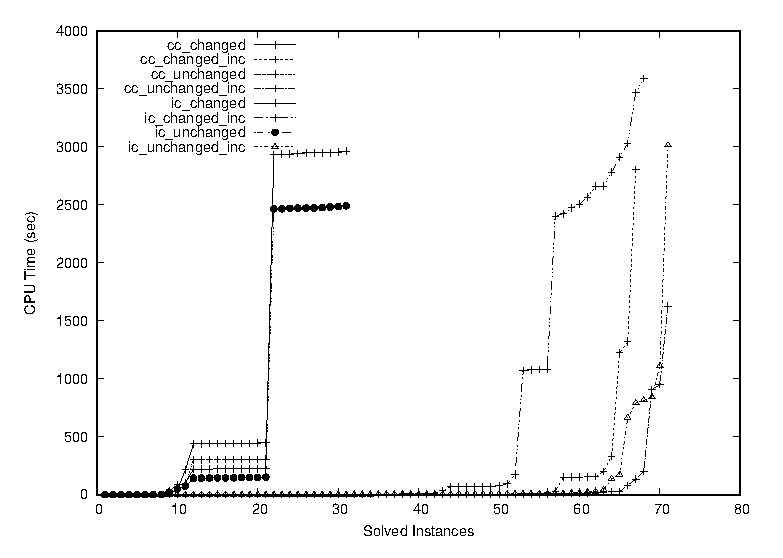
\includegraphics[scale=0.4]{fig/cactus.eps}
  \caption{基本符号化(コード~\ref{code:srf1.lp})と改良符号化(コード~\ref{code:srf2.lp})と
 発展符号化(コード~ \ref{code:srf3.lp})の比較} 
  \label{fig:cactus}
\end{figure*}
%%%%%%%%%%%%%%%%%%%%%%%%%%%%%%

%%%%%%%%%%%%%%%%%%%%%%%%%%%%%%
\begin{table*}[t]
  \caption{基本符号化(コード~\ref{code:srf1.lp})と改良符号化(コード~\ref{code:srf2.lp})と発展符号化(コード~ \ref{code:srf3.lp})の比較 (解けた問題数)} 
  \label{table:kibo}
  \centering
  \begin{tabular}[t]{rcr|c|ccc}
    \noalign{\hrule height 1pt}
    \multicolumn{3}{c|}{辺の数} & 問題数 & 基本符号化 & 改良符号化 & 発展符号化\\
    \noalign{\hrule height 1pt}
    %%%%%%%% 
       1 &~& 1000 & 30 & \textbf{30} & \textbf{30} & \textbf{30} \\ 
    1001 &~& 4000 & 20 & \textbf{20} & \textbf{20} & \textbf{20} \\ 
    4001 &~& 7000 & 11 & 9 & \textbf{10} & \textbf{10} \\ 
    7001 &~& 10000 & 8 & 4 & 6 & \textbf{8}  \\ 
    10001 &~& 20000 & 9 & 2 & 5 & \textbf{9} \\ 
    20001 &~& 30000 & 2 & 1 & \textbf{2} & \textbf{2} \\ 
    30001 &~& 40000 & 1 & 0 & 0 & \textbf{1} \\
    40001 &~& 50000 & 4 & 0 & 2 & \textbf{4} \\
    %%%%%%%% 合計
    \noalign{\hrule height 1pt}
    \multicolumn{3}{c|}{計} & 85 & 66 & 75 & \textbf{84} \\
    \noalign{\hrule height 1pt}
  \end{tabular}
\end{table*}
%%%%%%%%%%%%%%%%%%%%%%%%%%%%%%

%%%%%%%%%%%%%%%%%%%%%%%%%%%%%%
\begin{table*}[t]
  \centering
  \caption{配電網遷移問題のASP符号化(コード~\ref{code:pw-core})の実行結果}
  \label{table:core}
  \begin{tabular}{ccrrr}
 \rowcolor[RGB]{0,96,0}
\color{white}最短ステップ長 & \color{white}問題数 
     & \multicolumn{1}{c}{\color{white}シングルショット} 
         & \multicolumn{1}{c}{\color{white}マルチショット} 
             & \multicolumn{1}{c}{\color{white}シングル/マルチ} \\
 \rowcolor[RGB]{230,239,230}
1 & 6 & 1.677 & 1.035 & 1.620 \\
 \rowcolor[RGB]{196,230,196}
2 & 62 & 3.507 & 1.608 & 2.180 \\
 \rowcolor[RGB]{230,239,230}
3 & 189 & 6.089 & 2.155 & 2.826 \\
 \rowcolor[RGB]{196,230,196}
4 & 312 & 9.294 & 2.734 & 3.399 \\
 \rowcolor[RGB]{230,239,230}
5 & 280 & 13.338 & 3.361 & 3.968 \\
 \rowcolor[RGB]{196,230,196}
6 & 130 & 18.303 & 4.165 & 4.394 \\
 \rowcolor[RGB]{230,239,230}
7 & 21 & 24.483 & 5.086 & 4.814 \\
\noalign{\hrule height 0.5pt}
 \rowcolor[RGB]{196,230,196}
計 & 1000 & 76.691 & 20.114 & 3.807 \\
\end{tabular}


\end{table*}
%%%%%%%%%%%%%%%%%%%%%%%%%%%%%%

提案アプローチの有効性を評価するために,
節~\ref{chap:encode}と節~\ref{chap:core}の符号化に基づくソルバー
を開発し,実行実験を行った.

\textbf{根付き全域森問題.}
ベンチマークとしては,
DNET~\footnote{\url{https://github.com/takemaru/dnet}}
で公開されている配電網問題3問,および,
Graph Coloring and its Generalization~\footnote{\url{http://mat.tepper.cmu.edu/COLOR04/}}
で公開されているグラフ彩色問題をもとに生成した82問\footnote{%
グラフ彩色問題127問の中から,連結グラフで辺の数が50,000以下である
82問を使用した.根については全ノードの1/5をランダムに選んで使用した.
}を使用した.
ベンチマーク問題(計85問)の規模は,
ノード数11〜1406,辺の数16〜49629,根ノード数1〜281である.
%
ASPシステムには {\clingo}-5.4.0 (\textit{trendy})を使用し,
問題1問あたりの制限時間は1時間とした.
実験環境は,Mac mini,3.2 GHz Intel Core i7,64GB メモリである.

基本符号化と改良符号化と発展符号化の比較結果を
図~\ref{fig:cactus}に示す.
この図はカクタスプロットと呼ばれ,
縦軸がCPU時間,横軸が解けた問題数を表す.
グラフが下に寄るほどより高速に,右に寄るほどより多くの問題を解いたこと
を意味する.
図~\ref{fig:cactus}より,発展符号化は,他2つの符号化と比較して,より多く
の問題を高速に解いていることがわかる.

表~\ref{table:kibo}は,解けた問題数を,ベンチマーク問題に含まれる辺の数
で分類したものである.
発展符号化は,ほぼ全てのベンチマーク問題(85問中84問)が解けており,
大規模な問題に対する有効性が確認できた. 

\textbf{配電網遷移問題.}
ベンチマークとしては,DNETで公開されている実用規模の配電網問題
({\sf fukui-tepco},ノード数 432,根ノード数 72,電流上限 300)をベースにした.
この問題の実行可能解から,スタート状態を10個,ゴール状態を100個,
をランダムに選び,それらを組み合わせた計1000問の配電網遷移問題を生
成した.ASPシステムと実験環境は上と同じである.

配電網遷移問題のASP符号化(コード~\ref{code:pw-core.lp})の実行結果を
表~\ref{table:core}に示す.
左から順に,
問題名,
解を求めるまでのステップ長,解けた問題数,平均CPU時間を示している.
今回行った実行実験では,最長でステップ長が7の問題を解くことができた.


%%% Local Variables:
%%% mode: japanese-latex
%%% TeX-master: "paper"
%%% End:

%%%%%%%%%%%%%%%%%%%%%%%%%%%%%%%%%%%%%%%%%%%%%%%%%%%%%%%%%%% 
\chapter{結論}
%%%%%%%%%%%%%%%%%%%%%%%%%%%%%%%%%%%%%%%%%%%%%%%%%%%%%%%%%%

XXX

%%% Local Variables:
%%% mode: latex
%%% TeX-master: "paper"
%%% End:


\bibliographystyle {jssst}
\bibliography{bachelor,aisat}    % 参考文献リスト

\end{document}
%%%%%%%%%%%%%%%%%%%%%%%%%%%%%%%%%%%%%%%%%%%%%%%%%%%%%%%%%%

%%% Local Variables:
%%% mode: yatex
%%% TeX-master: t
%%% End:

